\documentclass[twoside]{book}

% Packages required by doxygen
\usepackage{fixltx2e}
\usepackage{calc}
\usepackage{doxygen}
\usepackage[export]{adjustbox} % also loads graphicx
\usepackage{graphicx}
\usepackage[utf8]{inputenc}
\usepackage{makeidx}
\usepackage{multicol}
\usepackage{multirow}
\PassOptionsToPackage{warn}{textcomp}
\usepackage{textcomp}
\usepackage[nointegrals]{wasysym}
\usepackage[table]{xcolor}

% Font selection
\usepackage[T1]{fontenc}
\usepackage[scaled=.90]{helvet}
\usepackage{courier}
\usepackage{amssymb}
\usepackage{sectsty}
\renewcommand{\familydefault}{\sfdefault}
\allsectionsfont{%
  \fontseries{bc}\selectfont%
  \color{darkgray}%
}
\renewcommand{\DoxyLabelFont}{%
  \fontseries{bc}\selectfont%
  \color{darkgray}%
}
\newcommand{\+}{\discretionary{\mbox{\scriptsize$\hookleftarrow$}}{}{}}

% Page & text layout
\usepackage{geometry}
\geometry{%
  a4paper,%
  top=2.5cm,%
  bottom=2.5cm,%
  left=2.5cm,%
  right=2.5cm%
}
\tolerance=750
\hfuzz=15pt
\hbadness=750
\setlength{\emergencystretch}{15pt}
\setlength{\parindent}{0cm}
\setlength{\parskip}{3ex plus 2ex minus 2ex}
\makeatletter
\renewcommand{\paragraph}{%
  \@startsection{paragraph}{4}{0ex}{-1.0ex}{1.0ex}{%
    \normalfont\normalsize\bfseries\SS@parafont%
  }%
}
\renewcommand{\subparagraph}{%
  \@startsection{subparagraph}{5}{0ex}{-1.0ex}{1.0ex}{%
    \normalfont\normalsize\bfseries\SS@subparafont%
  }%
}
\makeatother

% Headers & footers
\usepackage{fancyhdr}
\pagestyle{fancyplain}
\fancyhead[LE]{\fancyplain{}{\bfseries\thepage}}
\fancyhead[CE]{\fancyplain{}{}}
\fancyhead[RE]{\fancyplain{}{\bfseries\leftmark}}
\fancyhead[LO]{\fancyplain{}{\bfseries\rightmark}}
\fancyhead[CO]{\fancyplain{}{}}
\fancyhead[RO]{\fancyplain{}{\bfseries\thepage}}
\fancyfoot[LE]{\fancyplain{}{}}
\fancyfoot[CE]{\fancyplain{}{}}
\fancyfoot[RE]{\fancyplain{}{\bfseries\scriptsize Generated by Doxygen }}
\fancyfoot[LO]{\fancyplain{}{\bfseries\scriptsize Generated by Doxygen }}
\fancyfoot[CO]{\fancyplain{}{}}
\fancyfoot[RO]{\fancyplain{}{}}
\renewcommand{\footrulewidth}{0.4pt}
\renewcommand{\chaptermark}[1]{%
  \markboth{#1}{}%
}
\renewcommand{\sectionmark}[1]{%
  \markright{\thesection\ #1}%
}

% Indices & bibliography
\usepackage{natbib}
\usepackage[titles]{tocloft}
\setcounter{tocdepth}{3}
\setcounter{secnumdepth}{5}
\makeindex

% Hyperlinks (required, but should be loaded last)
\usepackage{ifpdf}
\ifpdf
  \usepackage[pdftex,pagebackref=true]{hyperref}
\else
  \usepackage[ps2pdf,pagebackref=true]{hyperref}
\fi
\hypersetup{%
  colorlinks=true,%
  linkcolor=blue,%
  citecolor=blue,%
  unicode%
}

% Custom commands
\newcommand{\clearemptydoublepage}{%
  \newpage{\pagestyle{empty}\cleardoublepage}%
}

\usepackage{caption}
\captionsetup{labelsep=space,justification=centering,font={bf},singlelinecheck=off,skip=4pt,position=top}

%===== C O N T E N T S =====

\begin{document}

% Titlepage & ToC
\hypersetup{pageanchor=false,
             bookmarksnumbered=true,
             pdfencoding=unicode
            }
\pagenumbering{alph}
\begin{titlepage}
\vspace*{7cm}
\begin{center}%
{\Large Telemetry System }\\
\vspace*{1cm}
{\large Generated by Doxygen 1.8.13}\\
\end{center}
\end{titlepage}
\clearemptydoublepage
\pagenumbering{roman}
\tableofcontents
\clearemptydoublepage
\pagenumbering{arabic}
\hypersetup{pageanchor=true}

%--- Begin generated contents ---
\chapter{Namespace Index}
\section{Namespace List}
Here is a list of all documented namespaces with brief descriptions\+:\begin{DoxyCompactList}
\item\contentsline{section}{\hyperlink{namespacedt}{dt} }{\pageref{namespacedt}}{}
\end{DoxyCompactList}

\chapter{Class Index}
\section{Class List}
Here are the classes, structs, unions and interfaces with brief descriptions\+:\begin{DoxyCompactList}
\item\contentsline{section}{\hyperlink{classdt_1_1data__reader}{dt\+::data\+\_\+reader} \\*Read data/signals from sensor }{\pageref{classdt_1_1data__reader}}{}
\end{DoxyCompactList}

\chapter{File Index}
\section{File List}
Here is a list of all documented files with brief descriptions\+:\begin{DoxyCompactList}
\item\contentsline{section}{src/\hyperlink{data__transfer_8cpp}{data\+\_\+transfer.\+cpp} \\*Implementation of data transfer functions and classes }{\pageref{data__transfer_8cpp}}{}
\item\contentsline{section}{src/\hyperlink{data__transfer_8hpp}{data\+\_\+transfer.\+hpp} \\*Functions and classes definition }{\pageref{data__transfer_8hpp}}{}
\end{DoxyCompactList}

\chapter{Namespace Documentation}
\hypertarget{namespacedt}{}\section{dt Namespace Reference}
\label{namespacedt}\index{dt@{dt}}
\subsection*{Classes}
\begin{DoxyCompactItemize}
\item 
class \hyperlink{classdt_1_1data__reader}{data\+\_\+reader}
\begin{DoxyCompactList}\small\item\em Read data/signals from sensor. \end{DoxyCompactList}\end{DoxyCompactItemize}
\subsection*{Functions}
\begin{DoxyCompactItemize}
\item 
\mbox{\Hypertarget{namespacedt_ab44fdb124992df044776c005d3e6b1ea}\label{namespacedt_ab44fdb124992df044776c005d3e6b1ea}} 
unsigned long \hyperlink{namespacedt_ab44fdb124992df044776c005d3e6b1ea}{operator\char`\"{}\char`\"{} \+\_\+ms} (unsigned long long time)
\begin{DoxyCompactList}\small\item\em A function for specifying time in milliseconds. \end{DoxyCompactList}\item 
void \hyperlink{namespacedt_a895a4305e8593c4428b867c1675a46fa}{encode\+\_\+msg} (String msg, int sig\+\_\+duration=20\+\_\+ms, int write\+\_\+pin=5)
\item 
\mbox{\Hypertarget{namespacedt_a5b66b3d9dbde9ddeacd2269ce71e7002}\label{namespacedt_a5b66b3d9dbde9ddeacd2269ce71e7002}} 
String {\bfseries decode\+\_\+msg} (int sig\+\_\+duration=20\+\_\+ms, int read\+\_\+pin=2)
\end{DoxyCompactItemize}


\subsection{Detailed Description}
A namespace for data transfer functions and classes. 

\subsection{Function Documentation}
\mbox{\Hypertarget{namespacedt_a895a4305e8593c4428b867c1675a46fa}\label{namespacedt_a895a4305e8593c4428b867c1675a46fa}} 
\index{dt@{dt}!encode\+\_\+msg@{encode\+\_\+msg}}
\index{encode\+\_\+msg@{encode\+\_\+msg}!dt@{dt}}
\subsubsection{\texorpdfstring{encode\+\_\+msg()}{encode\_msg()}}
{\footnotesize\ttfamily void dt\+::encode\+\_\+msg (\begin{DoxyParamCaption}\item[{String}]{msg,  }\item[{int}]{sig\+\_\+duration = {\ttfamily 20\+\_\+ms},  }\item[{int}]{write\+\_\+pin = {\ttfamily 5} }\end{DoxyParamCaption})}

Encode msg and send it to the receiver sensor.


\begin{DoxyParams}{Parameters}
{\em msg} & is the char sequence. \\
\hline
{\em sig\+\_\+duration} & is how long should be lasts signal. \\
\hline
{\em write\+\_\+to\+\_\+pin} & is a power supply to the sensor. \\
\hline
\end{DoxyParams}

\chapter{Class Documentation}
\hypertarget{classdt_1_1data__reader}{}\section{dt\+:\+:data\+\_\+reader Class Reference}
\label{classdt_1_1data__reader}\index{dt\+::data\+\_\+reader@{dt\+::data\+\_\+reader}}


Read data/signals from sensor.  




{\ttfamily \#include $<$data\+\_\+transfer.\+hpp$>$}

\subsection*{Public Member Functions}
\begin{DoxyCompactItemize}
\item 
bool \hyperlink{classdt_1_1data__reader_a4ca0a2870b3a03235d7804acf36672ed}{read\+\_\+data} (int signal\+\_\+pin, int sig\+\_\+duration=20\+\_\+ms)
\begin{DoxyCompactList}\small\item\em Read data from signal pin. \end{DoxyCompactList}\end{DoxyCompactItemize}
\subsection*{Static Public Member Functions}
\begin{DoxyCompactItemize}
\item 
\mbox{\Hypertarget{classdt_1_1data__reader_ab55bdd30fa1dd0d4fc5ec162e911d760}\label{classdt_1_1data__reader_ab55bdd30fa1dd0d4fc5ec162e911d760}} 
static \hyperlink{classdt_1_1data__reader}{data\+\_\+reader} \& {\bfseries instance} ()
\end{DoxyCompactItemize}


\subsection{Detailed Description}
Read data/signals from sensor. 

Read data/signals from sender sensor and translate it into bool. 

\subsection{Member Function Documentation}
\mbox{\Hypertarget{classdt_1_1data__reader_a4ca0a2870b3a03235d7804acf36672ed}\label{classdt_1_1data__reader_a4ca0a2870b3a03235d7804acf36672ed}} 
\index{dt\+::data\+\_\+reader@{dt\+::data\+\_\+reader}!read\+\_\+data@{read\+\_\+data}}
\index{read\+\_\+data@{read\+\_\+data}!dt\+::data\+\_\+reader@{dt\+::data\+\_\+reader}}
\subsubsection{\texorpdfstring{read\+\_\+data()}{read\_data()}}
{\footnotesize\ttfamily bool dt\+::data\+\_\+reader\+::read\+\_\+data (\begin{DoxyParamCaption}\item[{int}]{signal\+\_\+pin,  }\item[{int}]{sig\+\_\+duration = {\ttfamily 20\+\_\+ms} }\end{DoxyParamCaption})}



Read data from signal pin. 

Read data from signal pin and translate it into bool by specific time duration.


\begin{DoxyParams}{Parameters}
{\em signal\+\_\+pin} & just pin where we get this signals. \\
\hline
{\em sig\+\_\+duration} & is how long lasts signal. \\
\hline
\end{DoxyParams}


The documentation for this class was generated from the following files\+:\begin{DoxyCompactItemize}
\item 
src/\hyperlink{data__transfer_8hpp}{data\+\_\+transfer.\+hpp}\item 
src/\hyperlink{data__transfer_8cpp}{data\+\_\+transfer.\+cpp}\end{DoxyCompactItemize}

\chapter{File Documentation}
\hypertarget{data__transfer_8cpp}{}\section{src/data\+\_\+transfer.cpp File Reference}
\label{data__transfer_8cpp}\index{src/data\+\_\+transfer.\+cpp@{src/data\+\_\+transfer.\+cpp}}


Implementation of data transfer functions and classes.  


{\ttfamily \#include \char`\"{}data\+\_\+transfer.\+hpp\char`\"{}}\newline
Include dependency graph for data\+\_\+transfer.\+cpp\+:
\nopagebreak
\begin{figure}[H]
\begin{center}
\leavevmode
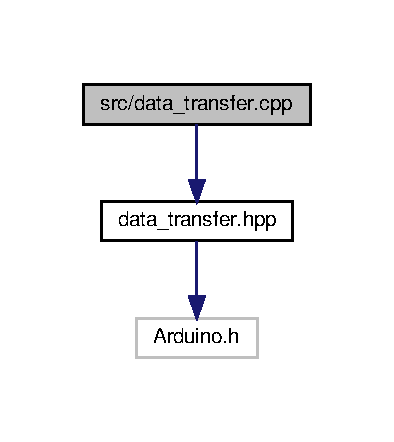
\includegraphics[width=189pt]{data__transfer_8cpp__incl}
\end{center}
\end{figure}


\subsection{Detailed Description}
Implementation of data transfer functions and classes. 


\hypertarget{data__transfer_8hpp}{}\section{src/data\+\_\+transfer.hpp File Reference}
\label{data__transfer_8hpp}\index{src/data\+\_\+transfer.\+hpp@{src/data\+\_\+transfer.\+hpp}}


Functions and classes definition.  


{\ttfamily \#include $<$Arduino.\+h$>$}\newline
Include dependency graph for data\+\_\+transfer.\+hpp\+:
\nopagebreak
\begin{figure}[H]
\begin{center}
\leavevmode
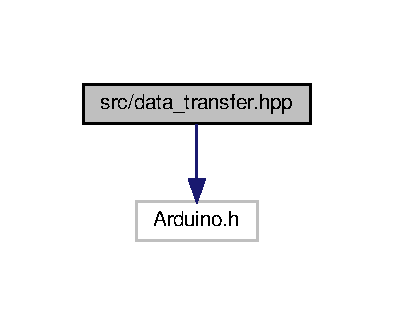
\includegraphics[width=189pt]{data__transfer_8hpp__incl}
\end{center}
\end{figure}
This graph shows which files directly or indirectly include this file\+:
\nopagebreak
\begin{figure}[H]
\begin{center}
\leavevmode
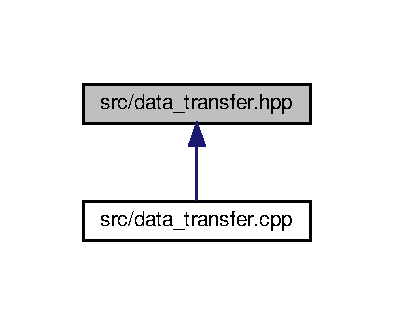
\includegraphics[width=189pt]{data__transfer_8hpp__dep__incl}
\end{center}
\end{figure}
\subsection*{Classes}
\begin{DoxyCompactItemize}
\item 
class \hyperlink{classdt_1_1data__reader}{dt\+::data\+\_\+reader}
\begin{DoxyCompactList}\small\item\em Read data/signals from sensor. \end{DoxyCompactList}\end{DoxyCompactItemize}
\subsection*{Namespaces}
\begin{DoxyCompactItemize}
\item 
 \hyperlink{namespacedt}{dt}
\end{DoxyCompactItemize}
\subsection*{Functions}
\begin{DoxyCompactItemize}
\item 
\mbox{\Hypertarget{namespacedt_ab44fdb124992df044776c005d3e6b1ea}\label{namespacedt_ab44fdb124992df044776c005d3e6b1ea}} 
unsigned long \hyperlink{namespacedt_ab44fdb124992df044776c005d3e6b1ea}{dt\+::operator\char`\"{}\char`\"{} \+\_\+ms} (unsigned long long time)
\begin{DoxyCompactList}\small\item\em A function for specifying time in milliseconds. \end{DoxyCompactList}\item 
void \hyperlink{namespacedt_a895a4305e8593c4428b867c1675a46fa}{dt\+::encode\+\_\+msg} (String msg, int sig\+\_\+duration=20\+\_\+ms, int write\+\_\+pin=5)
\item 
\mbox{\Hypertarget{namespacedt_a5b66b3d9dbde9ddeacd2269ce71e7002}\label{namespacedt_a5b66b3d9dbde9ddeacd2269ce71e7002}} 
String {\bfseries dt\+::decode\+\_\+msg} (int sig\+\_\+duration=20\+\_\+ms, int read\+\_\+pin=2)
\end{DoxyCompactItemize}


\subsection{Detailed Description}
Functions and classes definition. 


%--- End generated contents ---

% Index
\backmatter
\newpage
\phantomsection
\clearemptydoublepage
\addcontentsline{toc}{chapter}{Index}
\printindex

\end{document}
